\documentclass[a4paper, fontsize=11pt]{scrartcl} % A4 paper and 11pt font 
\usepackage[a4paper,left=3cm,right=2cm,top=2.5cm,bottom=2.5cm]{geometry}

\usepackage[T1]{fontenc} % Use 8-bit encoding that has 256 glyphs
\usepackage{fourier} % Use the Adobe Utopia font for the document - comment this line to return to the LaTeX default
\usepackage[spanish]{babel} % Spanish language/hyphenation
\selectlanguage{spanish}
\usepackage[utf8]{inputenc}
\usepackage{amsmath,amsfonts,amsthm} % Math packages
\usepackage{graphicx} % The graphicx package
\usepackage{placeins}
\usepackage{caption}
\usepackage{subcaption}


\usepackage{listings} % Insert Scripts
\usepackage{color} %red, green, blue, yellow, cyan, magenta, black, white
\definecolor{mygreen}{RGB}{28,172,0} % color values Red, Green, Blue
\definecolor{mylilas}{RGB}{170,55,241}

\lstset{language=Matlab,%
	%basicstyle=\color{red},
	breaklines=true,%
	morekeywords={matlab2tikz},
	keywordstyle=\color{blue},%
	morekeywords=[2]{1}, keywordstyle=[2]{\color{black}},
	identifierstyle=\color{black},%
	stringstyle=\color{mylilas},
	commentstyle=\color{mygreen},%
	showstringspaces=false,%without this there will be a symbol in the places where there is a space
	numbers=left,%
	numberstyle={\tiny \color{black}},% size of the numbers
	numbersep=9pt, % this defines how far the numbers are from the text
	emph=[1]{for,end,break},emphstyle=[1]\color{red}, %some words to emphasise
	%emph=[2]{word1,word2}, emphstyle=[2]{style},    
}

\usepackage{sectsty} % Allows customizing section commands
%\allsectionsfont{\centering \normalfont\scshape} % Make all sections centered, the default font and small caps

\usepackage{fancyhdr} % Custom headers and footers
\pagestyle{fancyplain} % Makes all pages in the document conform to the custom headers and footers
\fancyhead{} % No page header - if you want one, create it in the same way as the footers below
\fancyfoot[L]{} % Empty left footer
\fancyfoot[C]{} % Empty center footer
\fancyfoot[R]{\thepage} % Page numbering for right footer
\renewcommand{\headrulewidth}{0pt} % Remove header underlines
\renewcommand{\footrulewidth}{0pt} % Remove footer underlines
\setlength{\headheight}{13.6pt} % Customize the height of the header

\numberwithin{equation}{section} % Number equations within sections (i.e. 1.1, 1.2, 2.1, 2.2 instead of 1, 2, 3, 4)
\numberwithin{figure}{section} % Number figures within sections (i.e. 1.1, 1.2, 2.1, 2.2 instead of 1, 2, 3, 4)
\numberwithin{table}{section} % Number tables within sections (i.e. 1.1, 1.2, 2.1, 2.2 instead of 1, 2, 3, 4)

%\setlength\parindent{0pt} % Removes all indentation from paragraphs - comment this line for an assignment with lots of text

\newenvironment{myalign}{\par\nobreak\large\noindent\align}{\endalign} %Altering fontsize in equations globally

%----------------------------------------------------------------------------------------
%	TITLE SECTION
%----------------------------------------------------------------------------------------

\newcommand{\horrule}[1]{\rule{\linewidth}{#1}} % Create horizontal rule command with 1 argument of height

\title{	
	\normalfont \normalsize 
	\textsc{Master en Automática y Robótica - UPM} \\ [25pt] % Your university, school and/or department name(s)
	\horrule{0.5pt} \\[0.4cm] % Thin top horizontal rule
	\huge Identificación de Filtro con Ruido Blanco \\ % The assignment title
	\horrule{2pt} \\[0.5cm] % Thick bottom horizontal rule
}

\author{Jorge Camarero Vera - 07052} % Your name

\date{\normalsize\today} % Today's date or a custom date

\begin{document}
	\maketitle
	
	\section{Explicación de la tarea}
	
	Calcular la función de transferencia que contiene el bloque \textit{Ruido1} en el archivo \textit{sistema\_tema\_3y4} y calcula la varianza de los datos de entrada. 
	
	\begin{figure}[h!]
		\centering
		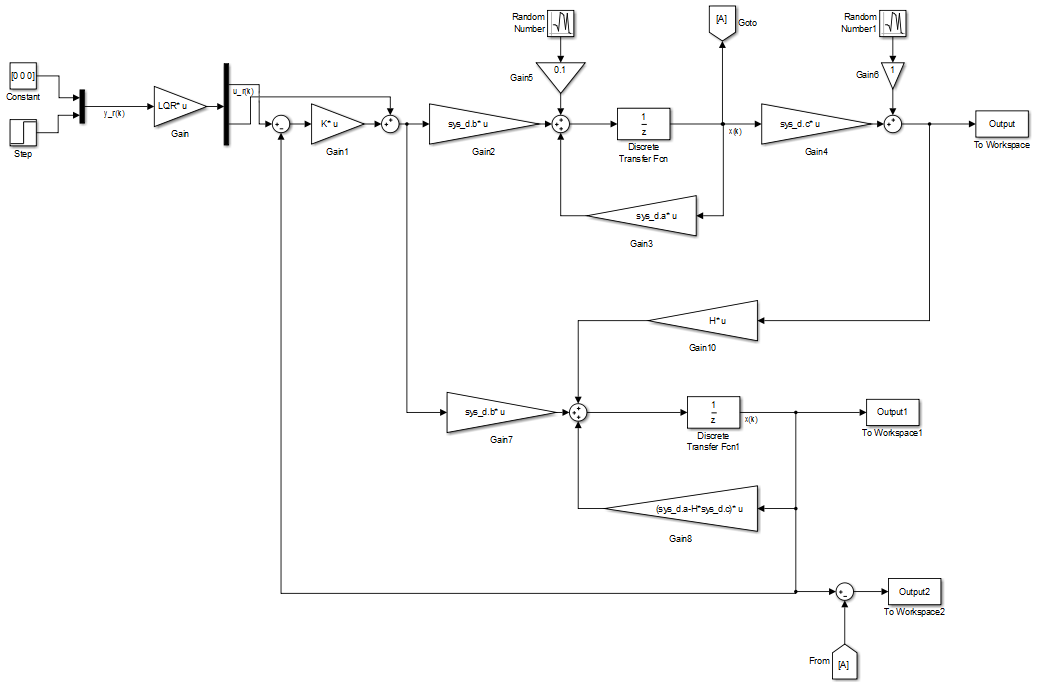
\includegraphics[width=1.0\linewidth]{images/model.PNG}
		\caption{Modelo inicial}
		\label{Modelo Inicial}
	\end{figure}
	\FloatBarrier
	
	\subsection{Presentación de los datos}
	
	Los valores de la señal de salida son los de la Figura \ref{Salida}.
	
	\begin{figure}[h!]
		\centering
		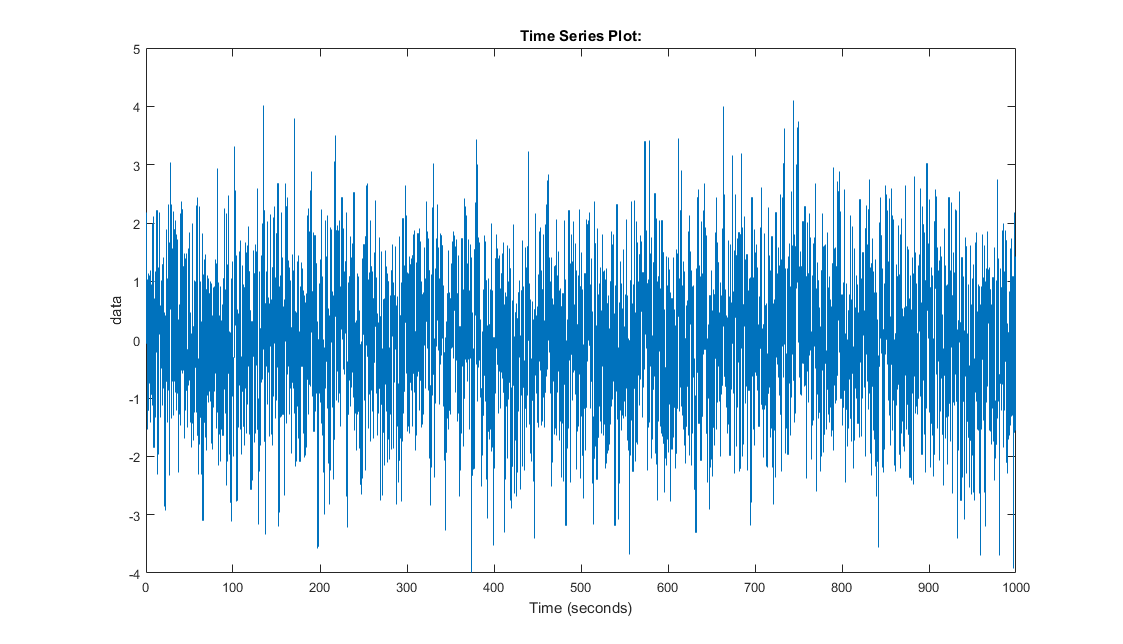
\includegraphics[width=1.0\linewidth]{images/output.PNG}
		\caption{Salida del bloque \textit{Ruido1}}
		\label{Salida}
	\end{figure}
	\FloatBarrier
	
	
	A partir de estos datos habrá que obtener la función de transferencia.

	\section{Identificación de la Función de Transferencia}	
	
	Para identificar la función de transferencia que produce esta señal se va a \textbf{estudiar en el dominio de la frecuencia}. Como la entrada en el bloque de \textit{Ruido1} es un ruido blanco entonces la salida será un proceso estocástico de segundo orden, es decir que la señal de salida tiene sus momentos de primer y segundo orden acotados. Por lo que el espectro de potencia de esta señal es la transformada de Fourier de su covarianza:
	
	\begin{myalign}
		S_x(\omega) = \sum_{k=-\infty}^{\infty}C_x(k)e^{-j\omega kT}= \left[ C_x(x) \right]_{z=e^{j\omega T}}
		\label{Fourier}
	\end{myalign}
	
	Entonces dado un proceso x(k), cuyo espectro de potencia es una función racional en $cos(\omega kT)$, existe un sistema lineal estable con función de transferencia $H(z)$ tal que alimentado con ruido blanco nos da como salida un proceso con el mismo espectro de potencia. Por tanto, se deberá proceder con la factorización espectral.
	
	Para las tareas de cálculo del algoritmo de factorización espectral he creado la clase de métodos estáticos, \textit{Spectral\_Analasys}, la cuál incluyo al final del presente documento.
	
	Primero se calcula la covarianza de la señal de la Figura \ref{Salida}, siguiendo la fórmula (\ref{covariance}). 
	
	\begin{myalign}
		C(i)\approx \dfrac{1}{N-1} \sum_{k=1}^{N}(x(k)-\bar{x})(x(k+i)-\bar{x})
		\label{covariance}
	\end{myalign}
	
	
	Para ello utilizo el método \textit{Covar(vect, num, index)} de la clase \textit{Spectral\_Analasys}, siendo \textit{vect} el vector con la señal, \textit{num} el número de valores de la señal a estudiar y \textit{index} el número de covarianzas que se quiere calcular.
	
	\begin{lstlisting}
	>> covariance = Spectral_Analysis.Covar(Salida.Data, length(Salida.Data)-1000,1000);
	\end{lstlisting}
	
	\begin{figure}[h!]
		\centering
		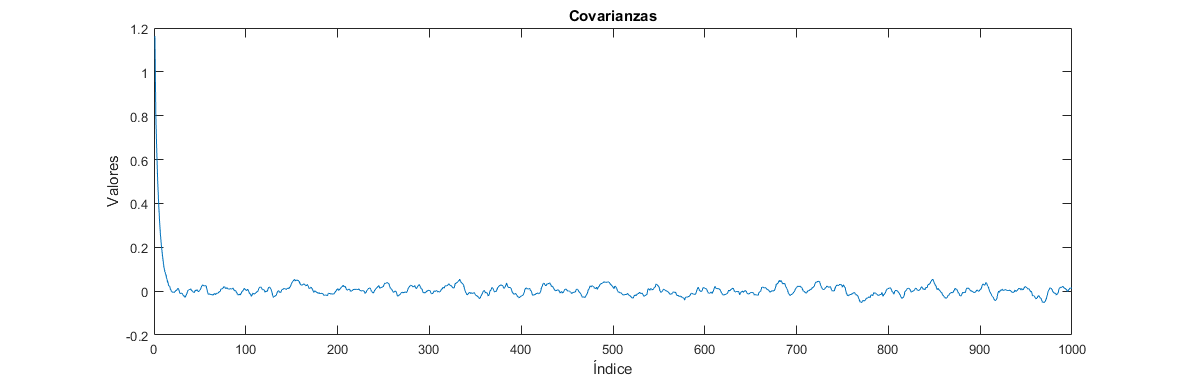
\includegraphics[width=1.0\linewidth]{images/covariances.PNG}
		\caption{Covarianzas calculadas}
		\label{Covariances Plot}
	\end{figure}
	\FloatBarrier
	
	Tras esto se calcula el espectro de potencia, fórmula (\ref{Spectral}).
	
	\begin{myalign}
		S(\omega) = C(0) + 2 \sum_{k=1}^{n_c}C(k)cos(\omega kT)
		\label{Spectral}
	\end{myalign}	
	
	Para ello se utiliza el método \textit{Fourier(vector)} de la clase \textit{Spectral\_Analasys}, siendo \textit{vector} en este caso el vector de covarianzas calculadas.
	
	\begin{lstlisting}
	>> Y = Spectral_Analysis.Fourier(covariance);
	\end{lstlisting}
	
	\begin{figure}[h!]
		\centering
		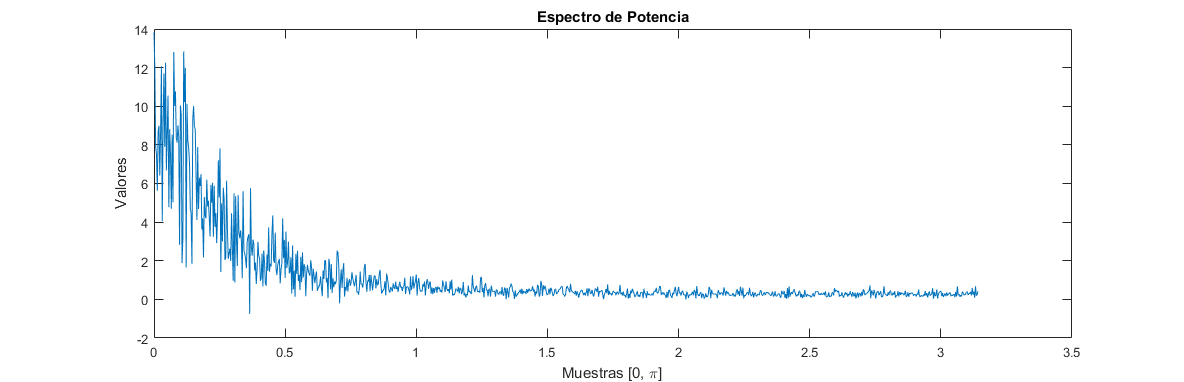
\includegraphics[width=1.0\linewidth]{images/spectral.PNG}
		\caption{Espectro de Potencia}
		\label{Spectral Analysis}
	\end{figure}
	\FloatBarrier
	
	Ahora habrá que aproximar el espectro por una función racional en cosenos, fórmula (\ref{Aprox Cos}) y calcular los parámetros mediante mínimos cuadrados.
	
	\begin{myalign}
		S(\omega) \approx \dfrac{b_0 + b_1 cos(\omega T)+b_2 cos(2\omega T)}{1 + a_1 cos(\omega T) + a_2 cos(2\omega T)}
		\label{Aprox Cos}
	\end{myalign}
	
	Para el cálculo de mínimos cuadrados habrá que minimizar la siguiente ecuación
	
	\[ J = \left\| \left[ \begin{array}{c}
	\vdots \\
	S(\omega_i) \\
	\vdots \\
	\end{array} \right] - \left[ \begin{array}{ccccc}
	\vdots & \vdots & \vdots & \vdots & \vdots \\
	1 & cos(\omega_i T) & cos(2 \omega_i T) & -S(\omega_i)cos(\omega_i T) & -S(\omega_i)cos(2\omega_i T) \\
	\vdots & \vdots & \vdots & \vdots & \vdots \\
	\end{array} \right] \cdot \left[ \begin{array}{c}
	b_0 \\
	b_1 \\
	b_2 \\
	a_1 \\
	a_2 \\ 
	\end{array} \right] \right\|^2  \] 
	
	Para el cálculo de mínimos cuadrados se ha creado el método \textit{Least\_Square(spectral, m, n)} de la clase \textit{Spectral\_Analasys}, en el que \textit{spectral} es el espectro de potencia, Figura \ref{Spectral Analysis}, m y n es el número de parámetros a calcular.
	
	\begin{lstlisting}
	>> p = Spectral_Analysis.Least_Square(Y(1:length(Y)),2,2);
	>> p =
	
	 0.3498
	-0.2471
	 0.0210
	-1.1215
	 0.1321
	\end{lstlisting}
	
	Al desarrollar el espectro de potencia en exponenciales y sustituyendo $z=e^{j\omega T}$, tenemos la siguiente ecuación:
	
	\begin{myalign}
		S(\omega) = \dfrac{b_2}{a_2}\dfrac{z^4 + \dfrac{b_1}{b_2}z^3+\dfrac{2b_0}{b_2}z^2+ \dfrac{b_1}{b_2}z + 1}{z^4 + \dfrac{a_1}{a_2}z^3+\dfrac{2}{a_2}z^2+ \dfrac{a_1}{a_2}z + 1}
	\end{myalign}
	
	Se factorizan los polinomios, para ello se utiliza el método \textit{CalculateRoots(p)} de la clase \textit{Spectral\_Analasys}.
	
	\begin{lstlisting}
	>> [num, den] = Spectral_Analysis.CalculateRoots(p)
	
	>> num =
	
		7.5743
		3.8021
		0.2630
		0.1320
		
	>> den =
	
		6.2921
		1.2087
		0.8273
		0.1589		
	\end{lstlisting}
	
	De estos valores se seleccionan para H(z) las de módulo menor o igual que 1, quedando en el numerador $0.2630$ y $0.1320$, y en el denominador $0.8273$ y $0.1589$. A partir de estos términos se forma:
	
	\begin{myalign}
		\begin{split}
			H(z) &= K\dfrac{\prod (z-z_i)}{\prod (p - p_i)} = K \dfrac{(z-0.2630)(z-0.1320)}{(z-0.8273)(z-0.1589)}\\
				 &= K \dfrac{z^2-0.3950z+0.0347}{z^2-0.9862+0.1315} 
		\end{split}
	\end{myalign}
	
	Como la entrada es ruido blanclo, $N(0,\sigma)$, entonces afectaría únicamente al cálculo del factor de ganancia.
	
	\begin{myalign}
		K^2 \dfrac{\prod z_i}{\prod p_i}\sigma = \dfrac{b_2}{a_2}
	\end{myalign}
	
	Si se fija $K = 1$, entonces,
	
	\begin{myalign}
			H(z) = \dfrac{z^2-0.3950z+0.0347}{z^2-0.9862+0.1315} 
	\end{myalign}
	 
	y quedará:
	
	\begin{myalign}
		\sigma = \sqrt{\dfrac{b_2}{a_2}\dfrac{\prod p_i}{\prod z_i}} = 0.7755
	\end{myalign}
	
	Se calcula, mediante el método CalculateWNoise(p,zeros,poles), en el que el vector $p$ son los parámetros calculados, $zeros$, los zeros seleccionado, y $poles$, los polos seleccionados. Finalmente la varianza del ruido blanco de entrada queda \textbf{$\sigma^2 = 0.6$}.
	
	\begin{lstlisting}
	>> [sigma, variance] = Spectral_Analysis.CalculateWNoise(p,[0.2630 0.1320],[0.8273 0.1589])
	
	sigma =
	
		0.7755
	
	
	variance =
	
		0.6014
	\end{lstlisting}
	
	
	
	Finalmente construimos un nuevo modelo, Figura \ref{New Model}, con la función de transferencia calculada, alimentada con una señal de entrada de ruido blanco con $\mu = 0$ y $\sigma^2 = 0.6$. Y obtenemos la Figura \ref{Comparative Output}. 
	
	\begin{figure}[h!]
		\centering
		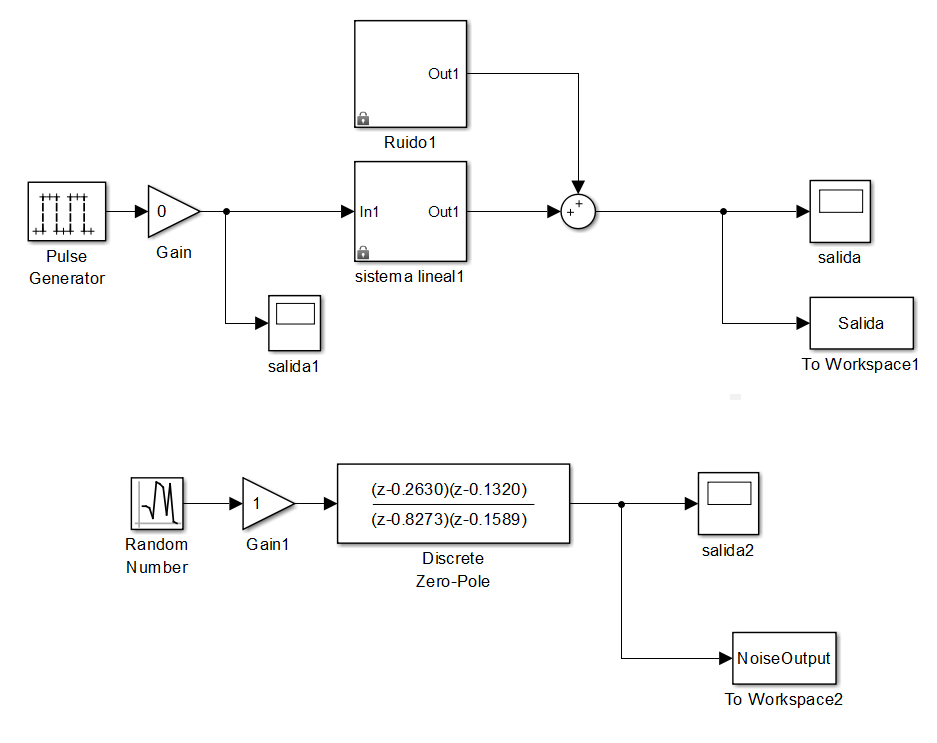
\includegraphics[width=1.0\linewidth]{images/newmodel.PNG}
		\caption{Modelo con la Función de Transferencia calculada.}
		\label{New Model}
	\end{figure}
	\FloatBarrier
	
	\begin{figure}[h!]
		\centering
		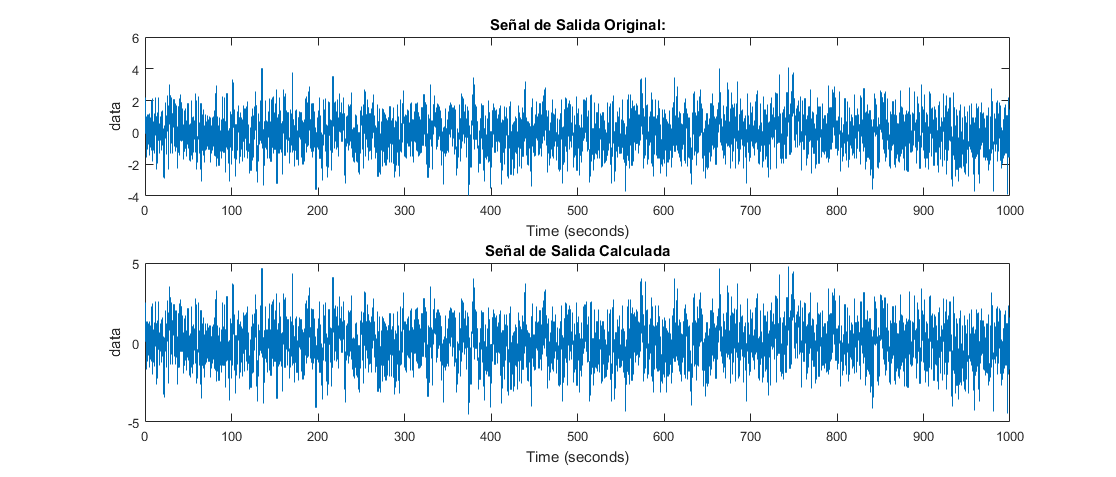
\includegraphics[width=1.0\linewidth]{images/comparative.PNG}
		\caption{Señal de salida original y calculada}
		\label{Comparative Output}
	\end{figure}
	\FloatBarrier
	
	Vemos que ambas señales de salida son iguales, por tanto queda definida la función de transferencia y la varianza del ruido blanco de entrada.
	
	\section{Identificar una función de transferencia más simple}
	
	Si aproximamos el espectro por una función racional en cosenos más simple, que (\ref{Aprox Cos}.
	
	\begin{myalign}
		S(\omega) \approx \dfrac{b_0 + b_1 cos(\omega T)}{1 + a_1 cos(\omega T)}
		\label{Aprox Cos Simple}
	\end{myalign}
	
	Para obtener los parámetros de esta función empleamos el método de mínimos cuadrados sobre la siguiente ecuación,
	
	\[ J = \left\| \left[ \begin{array}{c}
	\vdots \\
	S(\omega_i) \\
	\vdots \\
	\end{array} \right] - \left[ \begin{array}{ccc}
	\vdots & \vdots & \vdots \\
	1 & cos(\omega_i T) & -S(\omega_i)cos(\omega_i T) \\
	\vdots & \vdots & \vdots \\
	\end{array} \right] \cdot \left[ \begin{array}{c}
	b_0 \\
	b_1 \\
	a_1 \\
	\end{array} \right] \right\|^2  \] 
	
	Se hace el cálculo de mínimos cuadrados y se obtiene:
	
	\begin{lstlisting}
	>> p = Spectral_Analysis.Least_Square(Y(1:length(Y)),1,1)
		
	p =
	
	 0.3755
	-0.1717
	-0.9840
	\end{lstlisting}
	
	Al desarrollar el espectro de potencia, \ref{Aprox Cos Simple}, en exponenciales y sustituyendo $z=e^{j\omega T}$, tenemos la siguiente ecuación:
	
	\begin{myalign}
		S(\omega) = \dfrac{b_1}{a_1}\dfrac{z^2 + \dfrac{2b_0}{b_1}z+ 1}{z^2 + \dfrac{2}{a_1}z + 1}
	\end{myalign}
	
	Se factorizan los polinomios, para ello se utiliza el método \textit{CalculateRoots(p)}.
	
	\begin{lstlisting}
	>> [num, den] = Spectral_Analysis.CalculateRoots(p)
	
	num =
	
	4.1321
	0.2420
		
	den =
	
	1.1973
	0.8352
	\end{lstlisting}
	
	De estos valores se seleccionan para H(z) las de módulo menor o igual que 1, quedando en el numerado $0.2420$ y en el denominador $0.8352$. A partir de estos términos se forma:
	
	\begin{myalign}
			H(z) = K\dfrac{\prod (z-z_i)}{\prod (p - p_i)} = K \dfrac{z-0.2420}{z-0.8352}\\
	\end{myalign}
	
	Como la entrada es ruido blanco, $N(0,\sigma)$, entonces afectaría únicamente al cálculo  del factor de ganancia.
	
	\begin{myalign}
		K^2 \dfrac{\prod z_i}{\prod p_i}\sigma = \dfrac{b_1}{a_1}
	\end{myalign}
	
	Si se fija $K = 1$, entonces,
	
	\begin{myalign}
		H(z) = \dfrac{z-0.2420}{z-0.8352}
	\end{myalign}
	
	y quedará:
	
	\begin{myalign}
		\sigma = \sqrt{\dfrac{b_1}{a_1}\dfrac{\prod p_i}{\prod z_i}} = 0.7760
	\end{myalign}
	
	Se calcula, mediante el método \textit{CalculateWNoise(p,zeros,poles)} y la varianza queda la misma que en el apartado anterior, $\sigma^2 = 0.6$.
	
	\begin{lstlisting}
	>> [sigma, variance] = Spectral_Analysis.CalculateWNoise(p, 0.2420, 0.8352)
	
	sigma =
	
	0.7760	
		
	variance =
	
	0.6022
	\end{lstlisting}
	
	Finalmente construimos un nuevo modelo, Figura  \ref{New Model 2}, con la función de transferencia calculada, alimentada con una señal de entrada de ruido blanco con $\mu = 0$ y $\sigma^2 = 0.6$. Y obtenemos la Figura \ref{Comparative Output 2}.
	
	\begin{figure}[h!]
		\centering
		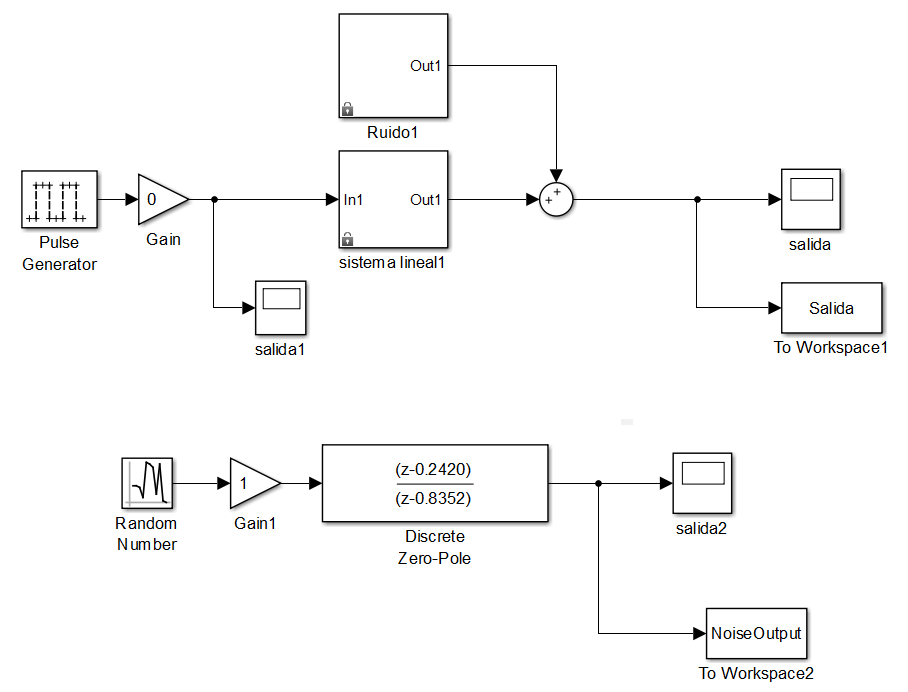
\includegraphics[width=1.0\linewidth]{images/newmodel2.PNG}
		\caption{Modelo con la nueva Función de Transferencia calculada.}
		\label{New Model 2}
	\end{figure}
	\FloatBarrier
	
	\begin{figure}[h!]
		\centering
		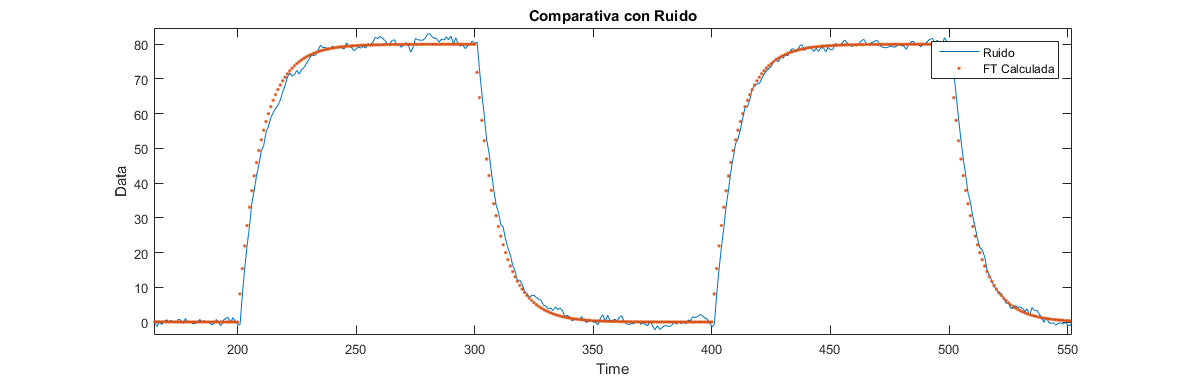
\includegraphics[width=1.0\linewidth]{images/comparative2.PNG}
		\caption{Señal de salida original y la nueva calculada}
		\label{Comparative Output 2}
	\end{figure}
	\FloatBarrier
	
	Vemos que ambas señales de salida son iguales, por tanto queda definida un nueva función de transferencia más simple y la varianza del ruido blanco sigue siendo la misma, $\sigma^2=0.6$. La función de transferencia es en $H(z)$: 
	
	\begin{myalign}
		H(z) = \dfrac{z-0.2420}{z-0.8352}
	\end{myalign}
	
	Y en $H(z^{-1})$:
	
	\begin{myalign}
		H(z^{-1}) = \dfrac{1-0.2420z^{-1}}{1-0.8352z^{-1}}
	\end{myalign}
	
	\section{Clase \textit{Spectral\_Analasys}}
	
	\lstinputlisting{scripts/Spectral_Analysis.m}
	
\end{document}